\documentclass{standalone}

\usepackage{TikzStyle}
\usepackage{mystyle}

\newcommand{\gpoint}[2]{%
\filldraw [gray] (#1,#2) circle [radius=2pt]
}

\begin{document}
    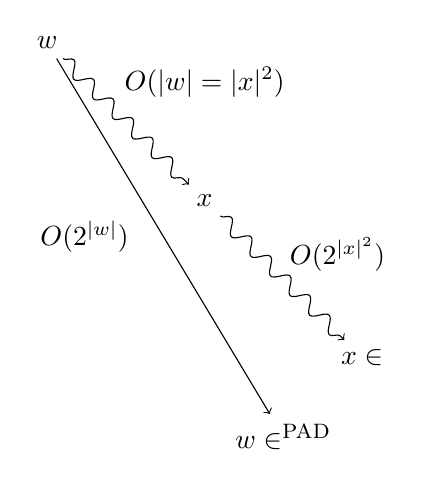
\begin{tikzpicture}
        \node (w) at (0,0) {$w$};
        \node (x) at (2,-2) {$x$};
        \node (xinL) at (4,-4) {$x \in \Lang$};
        \node (winLpad) at (3,-5) {$w \in \Lang^{\textsc{pad}}$};
        \draw[->,decorate,decoration=snake] (w) -- (x) node [pos=0.5,xshift=1cm,yshift=0.5cm]
        {$O(|w| = |x|^{2})$};
        \draw[->,decorate,decoration=snake] (x) -- (xinL) node [pos=0.5,xshift=0.7cm,yshift=0.3cm]
        {$O(2^{|x|^{2}})$};
        \draw[->] (w) -- (winLpad) node [pos=0.5,xshift=-1cm] {$O(2^{|w|})$};
    \end{tikzpicture}
\end{document}
